% Options for packages loaded elsewhere
\PassOptionsToPackage{unicode}{hyperref}
\PassOptionsToPackage{hyphens}{url}
%
\documentclass[
]{article}
\title{Einschätzung zu den Befindlichkeiten der Wirtschaft in den
Nachbarländern}
\author{Simon Wey}
\date{31 Oktober 2022}

\usepackage{amsmath,amssymb}
\usepackage{lmodern}
\usepackage{iftex}
\ifPDFTeX
  \usepackage[T1]{fontenc}
  \usepackage[utf8]{inputenc}
  \usepackage{textcomp} % provide euro and other symbols
\else % if luatex or xetex
  \usepackage{unicode-math}
  \defaultfontfeatures{Scale=MatchLowercase}
  \defaultfontfeatures[\rmfamily]{Ligatures=TeX,Scale=1}
\fi
% Use upquote if available, for straight quotes in verbatim environments
\IfFileExists{upquote.sty}{\usepackage{upquote}}{}
\IfFileExists{microtype.sty}{% use microtype if available
  \usepackage[]{microtype}
  \UseMicrotypeSet[protrusion]{basicmath} % disable protrusion for tt fonts
}{}
\makeatletter
\@ifundefined{KOMAClassName}{% if non-KOMA class
  \IfFileExists{parskip.sty}{%
    \usepackage{parskip}
  }{% else
    \setlength{\parindent}{0pt}
    \setlength{\parskip}{6pt plus 2pt minus 1pt}}
}{% if KOMA class
  \KOMAoptions{parskip=half}}
\makeatother
\usepackage{xcolor}
\IfFileExists{xurl.sty}{\usepackage{xurl}}{} % add URL line breaks if available
\IfFileExists{bookmark.sty}{\usepackage{bookmark}}{\usepackage{hyperref}}
\hypersetup{
  pdftitle={Einschätzung zu den Befindlichkeiten der Wirtschaft in den Nachbarländern},
  pdfauthor={Simon Wey},
  hidelinks,
  pdfcreator={LaTeX via pandoc}}
\urlstyle{same} % disable monospaced font for URLs
\usepackage[margin=1in]{geometry}
\usepackage{listings}
\newcommand{\passthrough}[1]{#1}
\lstset{defaultdialect=[5.3]Lua}
\lstset{defaultdialect=[x86masm]Assembler}
\usepackage{longtable,booktabs,array}
\usepackage{calc} % for calculating minipage widths
% Correct order of tables after \paragraph or \subparagraph
\usepackage{etoolbox}
\makeatletter
\patchcmd\longtable{\par}{\if@noskipsec\mbox{}\fi\par}{}{}
\makeatother
% Allow footnotes in longtable head/foot
\IfFileExists{footnotehyper.sty}{\usepackage{footnotehyper}}{\usepackage{footnote}}
\makesavenoteenv{longtable}
\usepackage{graphicx}
\makeatletter
\def\maxwidth{\ifdim\Gin@nat@width>\linewidth\linewidth\else\Gin@nat@width\fi}
\def\maxheight{\ifdim\Gin@nat@height>\textheight\textheight\else\Gin@nat@height\fi}
\makeatother
% Scale images if necessary, so that they will not overflow the page
% margins by default, and it is still possible to overwrite the defaults
% using explicit options in \includegraphics[width, height, ...]{}
\setkeys{Gin}{width=\maxwidth,height=\maxheight,keepaspectratio}
% Set default figure placement to htbp
\makeatletter
\def\fps@figure{htbp}
\makeatother
\setlength{\emergencystretch}{3em} % prevent overfull lines
\providecommand{\tightlist}{%
  \setlength{\itemsep}{0pt}\setlength{\parskip}{0pt}}
\setcounter{secnumdepth}{-\maxdimen} % remove section numbering
\usepackage{graphicx}
\usepackage{fancyhdr}
\usepackage{xcolor}
\usepackage{array}
\usepackage{tabularx}  
\newcolumntype{L}[1]{>{\raggedright\let\newline\\
\arraybackslash\hspace{0pt}}m{#1}}
\newcolumntype{C}[1]{>{\centering\let\newline\\
\arraybackslash\hspace{0pt}}m{#1}}
\newcolumntype{R}[1]{>{\raggedleft\let\newline\\
\arraybackslash\hspace{0pt}}m{#1}}
\newcolumntype{P}[1]{>{\raggedright\tabularxbackslash}p{#1}}

\pagestyle{fancy}
\usepackage{graphicx}
\usepackage{fancyhdr}
\pagestyle{fancy}
\usepackage[geometry]{ifsym}
\setlength{\footskip}{50pt}

\usepackage{fancyhdr}
\pagestyle{fancy}
% center of header
\fancyhf{}
\fancyhead[LE,RO]{Inflation: aktuelle Entwicklungen}
%\fancyhead[RO,LE]{}

% center of footer

\fancyfoot[LO]{
\includegraphics[width=4cm]{SAV.png}} %{\includegraphics[width=1.5cm,height=1.5cm,keepaspectratio]{logo.eps}}
\fancyfoot[RE]{
\includegraphics[width=4cm]{SAV.png}}


%\fancyfoot[LO,RE]{
\includegraphics[width=4cm]{SAV.png}{}}
% page number on the left of even pages and right of odd pages

\fancyfoot[C]{\thepage}
%\fancypagestyle{plain}{\pagestyle{fancy}}
%\fancyhead[C]{\ifnum\value{page}>1 center text \else \fi}
\usepackage{floatrow}
\floatsetup[figure]{capposition=top}
\usepackage{booktabs}
\usepackage{longtable}
\usepackage{array}
\usepackage{multirow}
\usepackage{wrapfig}
\usepackage{float}
\usepackage{colortbl}
\usepackage{pdflscape}
\usepackage{tabu}
\usepackage{threeparttable}
\usepackage{threeparttablex}
\usepackage[normalem]{ulem}
\usepackage{makecell}
\usepackage{xcolor}
\usepackage{amsmath}
\usepackage{caption}
\ifLuaTeX
  \usepackage{selnolig}  % disable illegal ligatures
\fi

\begin{document}
\maketitle
\begin{abstract}
Die steigenden Inflationsraten beschäftigen nicht nur Konsumentinnen und
Konsumenten, sondern auch die Politik, die sich überlegen muss, ob und
wie sie gegen den Kaufkraftverlust vorgehen will. Mit ihrer überraschend
starken Erhöhung des Leitzinses hat die Schweizerische Nationalbank
viele überrascht. Es bleiben die preistreibenden Entwicklungen als Folge
des Ukrainekriegs und der Corona-Pandemie, wobei diese die
zugrundeliegende Teuerung aufgrund der expansiven Geldpolitik der
Notenbanken überlagern. Eine vergleichbare Situation war die «Great
depression» in den 70er-Jahren. Eine Mehrheit der von NZZ und KOF
befragten Ökonomen geht von einem temporären Anstieg der Inflation aus.
Der Spielraum für Lohnerhöhungen bleibt überschaubar, denn auch die
Unternehmen kämpfen beim Bezug von Vorprodukten mit den höheren Preisen.
Dies nagt an der Marge und somit am Spielraum für Lohnerhöhungen.
Daneben kühlt sich auch die wirtschaftliche Entwicklung ab, etwa
aufgrund der zunehmend restriktiveren Geldpolitik, des Ukrainie-Kriegs
oder der nach wie vor schwierigen Covid-Situation in China.
\end{abstract}

\renewcommand{\figurename}{Abbildung} 
\fontsize{13}{16}

\selectfont

\hypertarget{einschuxe4tzung-zur-gesamtwirtschaftlichen-entwicklung-sowie-in-ausguxe4hlten-branchen-short-term-business-statistics}{%
\subsection{Einschätzung zur gesamtwirtschaftlichen Entwicklung sowie in
ausgählten Branchen (Short term business
statistics)}\label{einschuxe4tzung-zur-gesamtwirtschaftlichen-entwicklung-sowie-in-ausguxe4hlten-branchen-short-term-business-statistics}}

Die Berechnung des Economic Sentiment Indicators (ESI) der Schweiz lehnt
sich an die Berechnungsmethode der EU-Kommission. Die Europäische Union
berechnet diesen Indikator für alle ihre Mitgliederländer sowie für
Aggregate der EU mit unterschiedlicher Länderzusammensetzung. Die
Gewichtung der Umfragen unterschiedlicher Branchen wird im Indikator wie
folgt gewichtet:

\begin{itemize}
\tightlist
\item
  Verarbeitendes Gewerbe (40\%)
\item
  Baugewerbe (5\%)
\item
  Detailhandel (5\%)
\item
  Übrige Dienstleistungen (30\%)
\item
  Konsumentenumfrage (20\%)
\end{itemize}

Der ESI bildet die Einschätzungen von Wirtschaftsakteuren zur aktuellen
und zukünftigen wirtschaftlichen Entwicklung ab. Die Gewichtung richtet
sich nach den zwei Kriterien der Repräsentativität der Branche und deren
Einfluss bei der Voraussage des BIP-Wachstums. Die fünf im ESI
verwendeten Indikatoren bilden die Wahrnehmungen und Erwartungen der
Entwicklungen in den jeweiligen Branchen in einem komprimierten Index
ab. Die Berechnung der Indikatoren erfolgt basierend auf dem einfachen
arithmetischen Durchschnitt der saisonbereinigten Salden zu ausgewählten
Fragestellungen aus dem gesamten Fragekatalog. Um die
gesamtwirtschaftliche Entwicklung zu verfolgen wird der ESI als Aggregat
von verschiedenen Indikatoren gebildet. Die Indikatoren der EU-28 und
der Eurozone werden als gewichteter Durchschnitt der Indikatoren aus den
Ländern gebildet. Dabei bildet das jeweilige Gewicht der Länder deren
relative Grösse im entsprechenden Jahr und den relevanten Branchen und
Indikatoren. Die Publikation des ESI sowie der branchenspezifischen
Indikatoren erfolgt monatlich durch die EU-Kommission und die
Konjunkturforschungsstelle der ETH (KOF) für den Indikator in der
Schweiz.

Die
\href{https://ec.europa.eu/eurostat/statistics-explained/index.php?title=Short-term_business_statistics_and_the_economic_sentiment_indicator}{EU-Kommission}
publiziert neben dem ESI auch noch Vertrauensindikatoren für die
Industrie, das Baugewerbe, den Detailhandel, die Dienstleistungen, den
Finanzsektor sowie die Konsumentenstimmung. Die Erfassung der Zeitreihen
startet im Jahr 1985. Ein wichtiger Vorteil der Indikatoren ist die
präzisen Einschätzungen der zukünftigen wirtschaftlichen Entwicklung.
Die Präzision der Prgnosen lässt sich mit einer Gegenüberstellung mit
den später publizierten realen Daten vergleichen.

\hypertarget{kof-konjunkturbarometer}{%
\section{KOF-Konjunkturbarometer}\label{kof-konjunkturbarometer}}

Seit seinem Bestehen lassen sich vom Konjunkturbarometer der KOF
frühzeitige und zuverlässige Informationen zur konjunkturellen
Entwicklung der Schweiz in der nahen Zukunft ablesen. Das
Konjunkturbarometer der Konjunkturforschungsstelle der ETH (KOF) wird
auf einer durch die
KOF\href{https://kof.ethz.ch/prognosen-indikatoren/indikatoren/kof-konjunkturbarometer.html}{KOF}
berechneten Referenzreihe und der Vormonatsveränderung des BIP
berechnet. Letztere wird mittels Quartalisierung der Schweizer BIP-Daten
des Bundesamtes für Statistik und dessen Bereinigung um die Effekte
grosser internationaler Sportanlässe durch das Staatssekratariat für
Wirtschaft berechnet.

Ziel des Barometers ist, die aktuelle Schweizer Konjunkturentwicklung
möglichst zeitnah zu prognostizieren. Aus über 500 Indikatoren werden
zur Bildung des Barometers jene herangezogen, die zum einen eine
ökonomisch plausible Einflussnahme auf die Konjunktur haben und zum
anderen die Kombination aus Mindestvorlauf und Korrelation zur
Referenzreihe aufweisen. Auf Glättungen des Indikators, wie dies früher
noch der Fall war, wird inzwischen verzichtet. Dies erhöht die
Aussagekraft.

\begin{figure}[] \centering
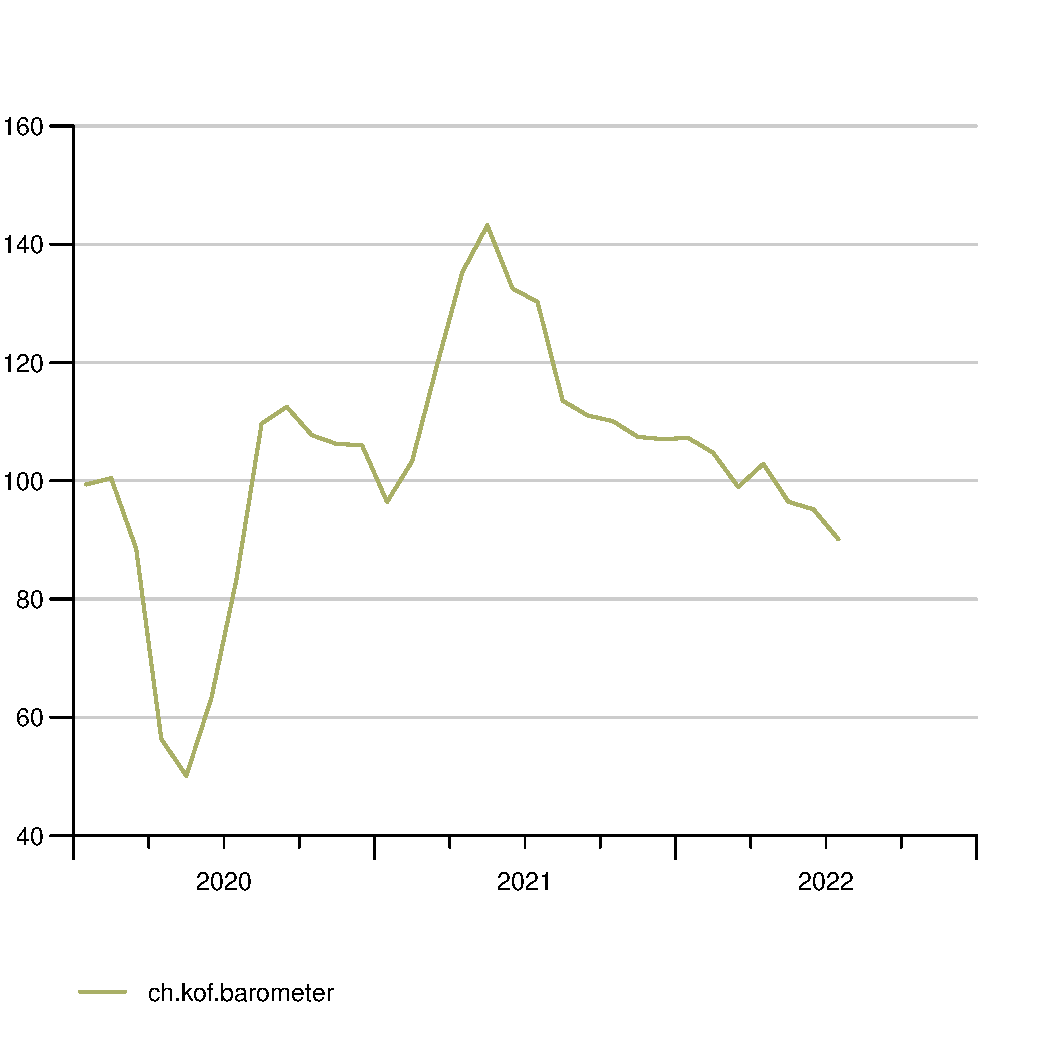
\includegraphics[trim={0 2.5cm 0 0cm },clip,width=.8\textwidth]
{/Users/simonwey/Repos/Foreign_economics/Graphics/baro.pdf}
\caption{KOF-Konjunkturbarometer mit aktuellem Wert im Oktober von 90.9.} 
\label{Inf_M_W}
\end{figure}

\begin{longtable}{lrr}
\caption*{
{\large KOF-Bartmeter. \emph{Quelle:} KOF}
} \\ 
\toprule
\textbf{Stand} & \textbf{Wert} & \textbf{Delta (Vormonat)} \\ 
\midrule
Oktober & $90.9$ & $-1.3$ \textcolor{green}{\FilledSmallTriangleDown} \\ 
\bottomrule
\end{longtable}

\begin{longtable}[]{@{}lll@{}}
\caption{KOF-Konjunkturbarometer, letzte Werte. Quelle:
KOF}\tabularnewline
\toprule
\textbf{Monat} & \textbf{September} & \textbf{Oktober} \\
\midrule
\endfirsthead
\toprule
\textbf{Monat} & \textbf{September} & \textbf{Oktober} \\
\midrule
\endhead
\textbf{KOF-Konjunktur-Barometer} & 92.3 & 90.9 \\
\bottomrule
\end{longtable}

\hypertarget{hallo}{%
\section{hallo}\label{hallo}}

A confidence indicator is a statistical indicator based on the results
from business surveys interrogating enterprises on their current
economic situation and their expectations about future developments.
Five separate confidence indicators are produced, for industry,
construction, services, retail trade and consumers.

A confidence indicator is a statistical indicator based on the results
from business surveys interrogating enterprises on their current
economic situation and their expectations about future developments.
Five separate confidence indicators are produced, for industry,
construction, services, retail trade and consumers. A confidence
indicator is a statistical indicator based on the results from business
surveys interrogating enterprises on their current economic situation
and their expectations about future developments. Five separate
confidence indicators are produced, for industry, construction,
services, retail trade and consumers.

A confidence indicator is a statistical indicator based on the results
from business surveys interrogating enterprises on their current
economic situation and their expectations about future developments.
Five separate confidence indicators are produced, for industry,
construction, services, retail trade and consumers.

A confidence indicator is a statistical indicator based on the results
from business surveys interrogating enterprises on their current
economic situation and their expectations about future developments.
Five separate confidence indicators are produced, for industry,
construction, services, retail trade and consumers.

\begin{figure}[] \centering
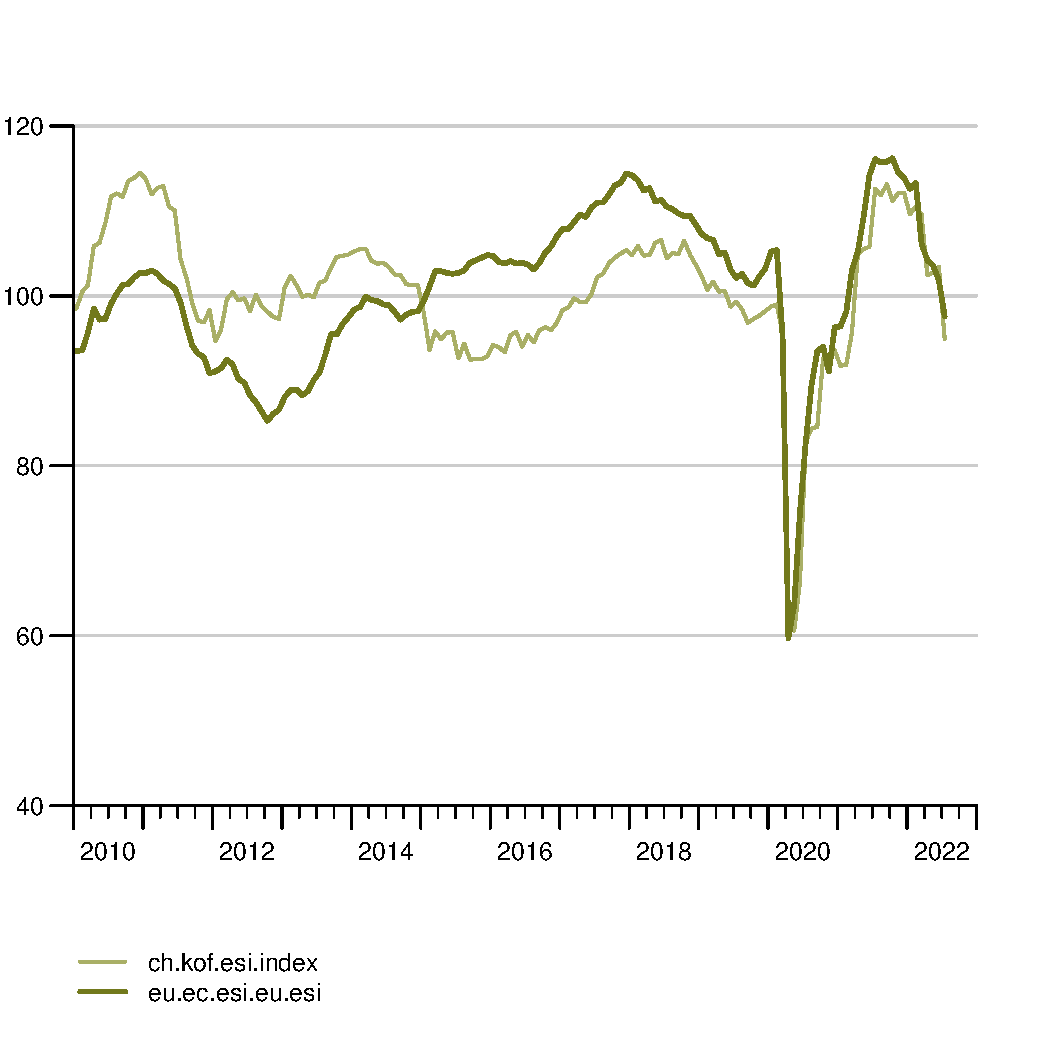
\includegraphics[trim={0 0cm 0 0cm },clip,width=.8\textwidth]
{/Users/simonwey/Repos/Foreign_economics/Graphics/ESI.pdf}
\caption{Economic Sentiment Indicator Schweiz und EU} 
\label{Inf_M_W}
\end{figure}

\begin{longtable}[]{@{}lll@{}}
\caption{ESI, letzte Werte. Quelle: KOF}\tabularnewline
\toprule
\textbf{Monat} & \textbf{August} & \textbf{September} \\
\midrule
\endfirsthead
\toprule
\textbf{Monat} & \textbf{August} & \textbf{September} \\
\midrule
\endhead
\textbf{ESI Schweiz} & 92.9 & 88.7 \\
------------- & ------------- & ------------- \\
\textbf{ESI EU} & 92.4 & 90.9 \\
\bottomrule
\end{longtable}

\begin{figure}[h] \centering
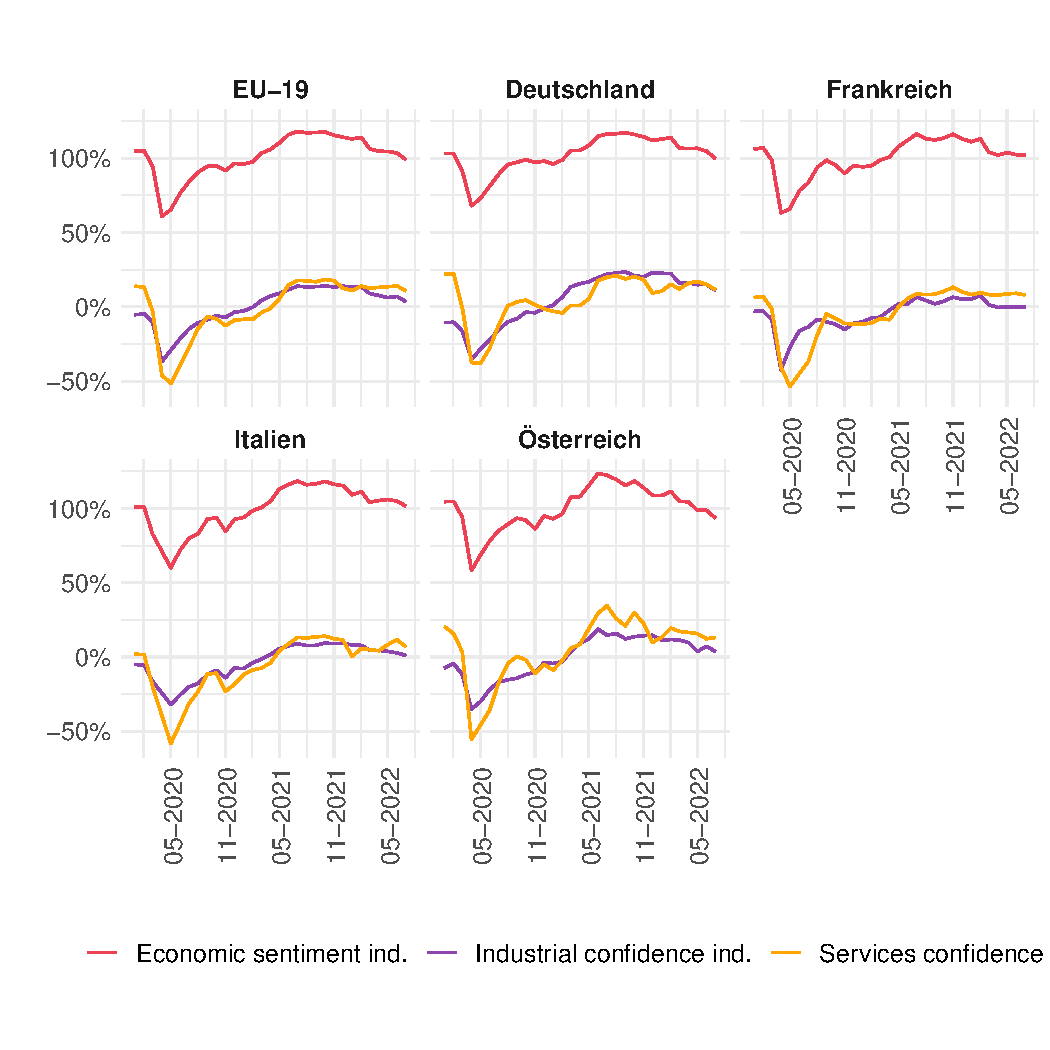
\includegraphics[trim={0 0cm 0 0cm },clip,width=\textwidth]{/Users/simonwey/Repos/Foreign_economics/Graphics/wrap_ESI.pdf}
\caption{Einschätzungen zur wirtschaftlichen Lage in der Gesamtwirtschaft und den Sektoren} 
\label{Inf_M_W}
\end{figure}

\begin{longtable}[]{@{}lll@{}}
\caption{Einschätzung zur wirtschaftlichen Lage in den entsprechenden
Ländern. Quelle: Eurostat}\tabularnewline
\toprule
\textbf{Wirtsch. Lage} & \textbf{September} & \textbf{Oktober} \\
\midrule
\endfirsthead
\toprule
\textbf{Wirtsch. Lage} & \textbf{September} & \textbf{Oktober} \\
\midrule
\endhead
\textbf{EU-19} & 93.6 & 92.5 \\
\textbf{Deutschland} & 91.9 & 90.9 \\
\textbf{Frankreich} & 96.2 & 96.2 \\
\textbf{Italien} & 95.9 & 95 \\
\textbf{Österreich} & 86.5 & 84.5 \\
\bottomrule
\end{longtable}

\begin{tabular}{|c *{8}{|c{2cm}}|} \cline{2-7}
    \multicolumn{1}{c|}{} & \multicolumn{6}{c|}{\textbf{Einschätzungen}} \\ \cline{2-7}
    \multicolumn{1}{c|}{} & \multicolumn{2}{c|}{\textbf{Wirtsch. Lage}} & \multicolumn{2}{c|}{\textbf{Ind.
Vertrauensind.}} & \multicolumn{2}{c|}{\textbf{DL
 Vertrauensind.}} \\ \hline
    \textbf{Land}  & September & Oktober & September & Oktober & September & Oktober \\ 
  \hline
EU-19 & 93.60 & 92.50 & -0.30 & -1.20 & 4.40 & 1.80 \\ 
   \hline
Deutschland & 91.90 & 90.90 & 4.00 & 2.90 & 3.60 & 0.50 \\ 
   \hline
Frankreich & 96.20 & 96.20 & -6.70 & -6.80 & 4.60 & 4.90 \\ 
   \hline
Italien & 95.90 & 95.00 & -3.80 & -4.40 & 0.50 & 1.10 \\ 
   \hline
Österreich & 86.50 & 84.50 & -3.60 & -6.60 & 0.90 & -0.40 \\ 
   \hline
\end{tabular}

\begin{tabular}{|c *{8}{|c{2cm}}|} \cline{2-3}
    \multicolumn{1}{c|}{} & \multicolumn{2}{c|}{\textbf{Wirtsch. Lage}} \\ \hline     \textbf{Land}  & September & Oktober \\ 
  \hline
EU-19 & 93.60 & 92.50 \\ 
   \hline
Deutschland & 91.90 & 90.90 \\ 
   \hline
Frankreich & 96.20 & 96.20 \\ 
   \hline
Italien & 95.90 & 95.00 \\ 
   \hline
Österreich & 86.50 & 84.50 \\ 
   \hline
\end{tabular}

\hypertarget{industrie}{%
\subsection{Industrie}\label{industrie}}

\begin{figure}[h] \centering
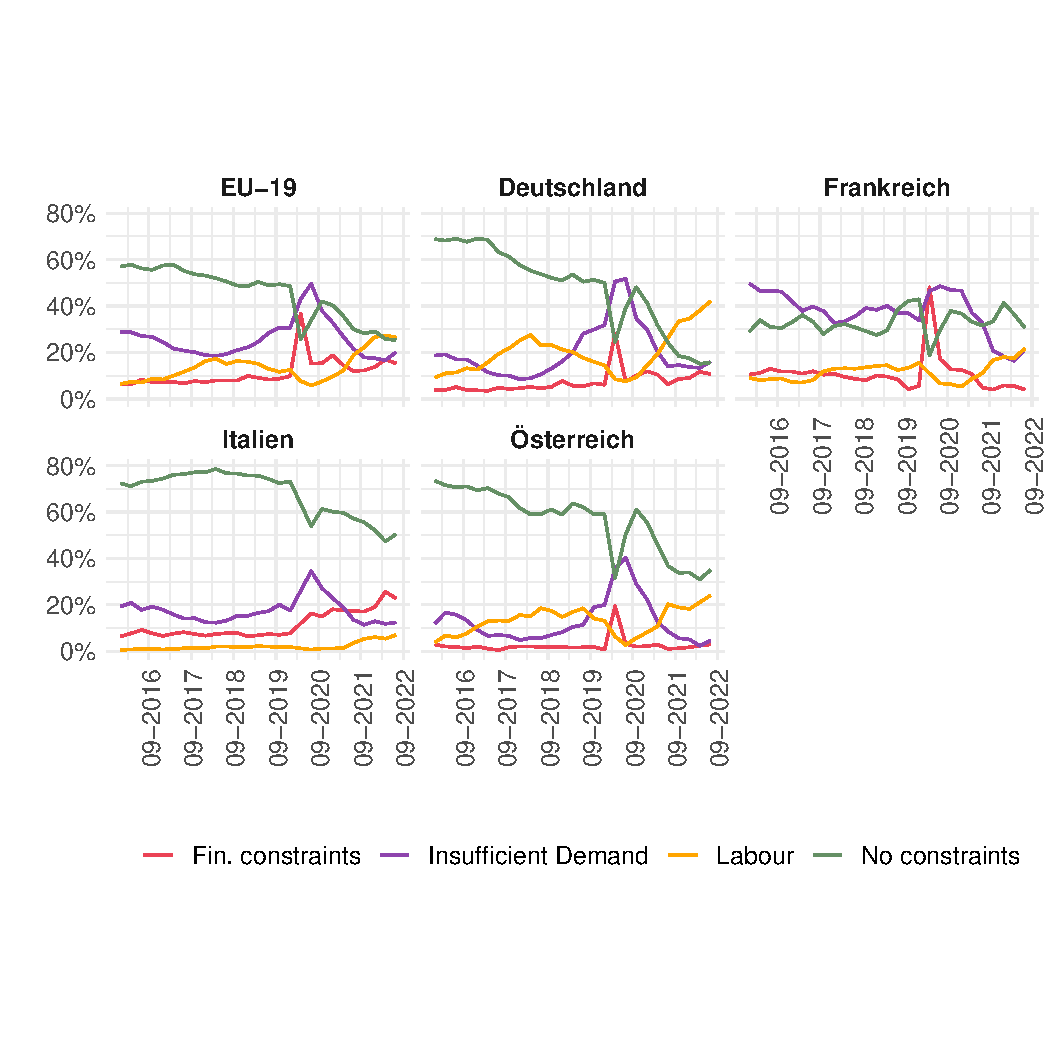
\includegraphics[trim={0 2.5cm 0 0cm },clip,width=\textwidth]{/Users/simonwey/Repos/Foreign_economics/Graphics/wrap_Hin_i.pdf}
\caption{Industrie: Hemmnisse in der Produktion} 
\label{Inf_M_W}
\end{figure}

\begin{tabular}{|c *{8}{|c{2cm}}|} \cline{2-7}
    \multicolumn{1}{c|}{} & \multicolumn{6}{c|}{\textbf{Einschätzungen Hemmnisse}} \\ \cline{2-7}
    \multicolumn{1}{c|}{} & \multicolumn{2}{c|}{\textbf{Arbeitskräftemangel}} & \multicolumn{2}{c|}{\textbf{Keine}} & \multicolumn{2}{c|}{\textbf{Andere}} \\ \hline
    \textbf{Land}  & 2022Q3 & 2022Q4 & 2022Q3 & 2022Q4 & 2022Q3 & 2022Q4 \\ 
  \hline
EU-19 & 26.40 & 26.40 &  &  &  &  \\ 
   \hline
Deutschland & 41.60 & 40.60 &  &  &  &  \\ 
   \hline
Frankreich & 21.00 & 20.20 &  &  &  &  \\ 
   \hline
Italien & 7.00 & 5.60 &  &  &  &  \\ 
   \hline
Österreich & 24.00 & 22.00 &  &  &  &  \\ 
   \hline
\end{tabular}

\hypertarget{dienstleistungen}{%
\subsection{Dienstleistungen}\label{dienstleistungen}}

\begin{figure}[] \centering
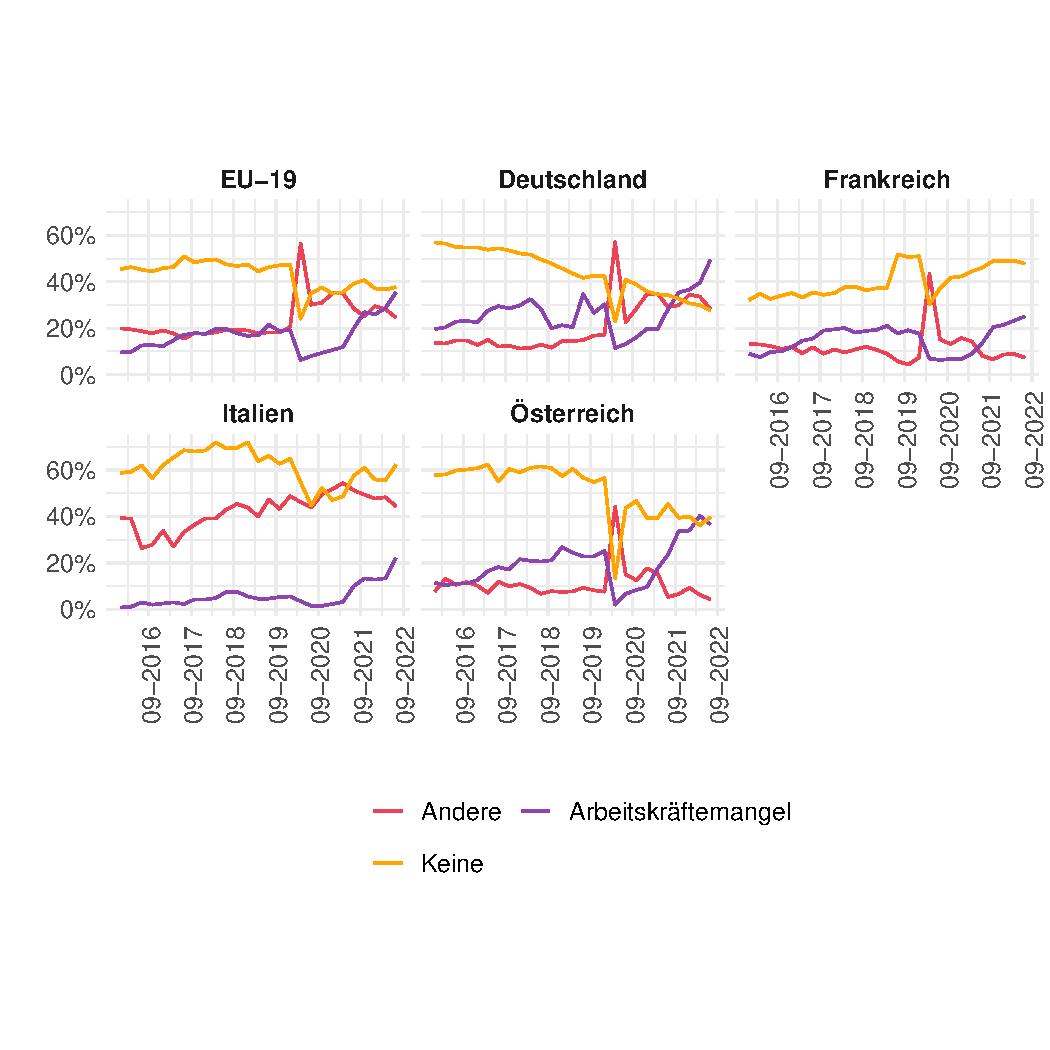
\includegraphics[trim={0 2.5cm 0 0cm },clip,width=\textwidth]
{/Users/simonwey/Repos/Foreign_economics/Graphics/wrap_Hin_s.pdf}
\caption{Dienstleistungen: Hemmnisse beim Erbringen von Dienstleistungen} 
\label{Inf_M_W}
\end{figure}

\begin{tabular}{|c *{8}{|c{2cm}}|} \cline{2-7}
    \multicolumn{1}{c|}{} & \multicolumn{6}{c|}{\textbf{Einschätzungen Hemmnisse}} \\ \cline{2-7}
    \multicolumn{1}{c|}{} & \multicolumn{2}{c|}{\textbf{Arbeitskräftemangel}} & \multicolumn{2}{c|}{\textbf{Keine}} & \multicolumn{2}{c|}{\textbf{Andere}} \\ \hline
    \textbf{Land}  & 2022Q3 & 2022Q4 & 2022Q3 & 2022Q4 & 2022Q3 & 2022Q4 \\ 
  \hline
EU-19 & 35.30 & 30.60 &  &  &  &  \\ 
   \hline
Deutschland & 49.40 & 41.30 &  &  &  &  \\ 
   \hline
Frankreich & 24.90 & 25.10 &  &  &  &  \\ 
   \hline
Italien & 22.10 & 15.80 &  &  &  &  \\ 
   \hline
Österreich & 36.40 & 32.10 &  &  &  &  \\ 
   \hline
\end{tabular}

\begin{figure}[] \centering
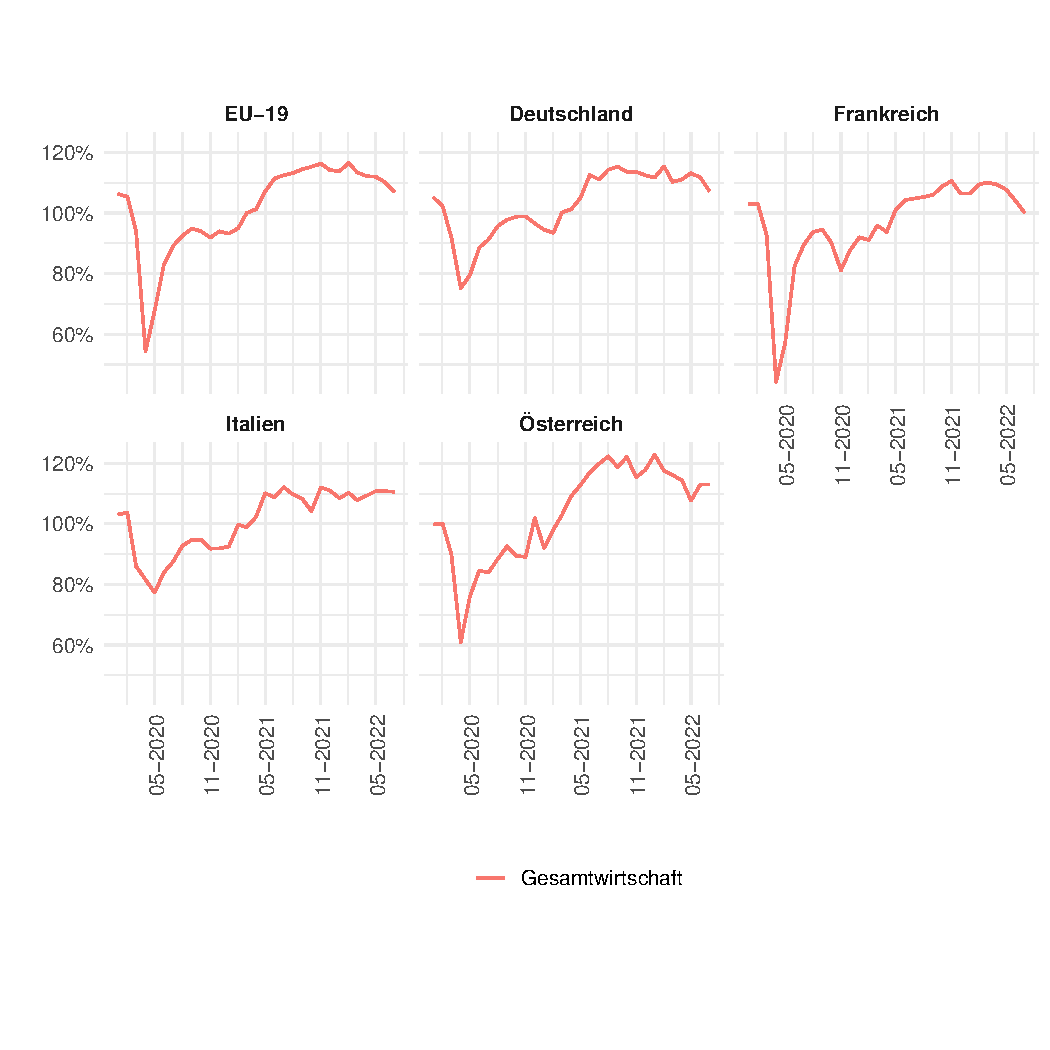
\includegraphics[trim={0 2.5cm 0 0cm },clip,width=\textwidth]
{/Users/simonwey/Repos/Foreign_economics/Graphics/BSC.pdf}
\caption{Gesamtwirtschaft: Beschäftigungsaussichten nächste 3 Mt.} 
\label{Inf_M_W}
\end{figure}

\begin{figure}[] \centering
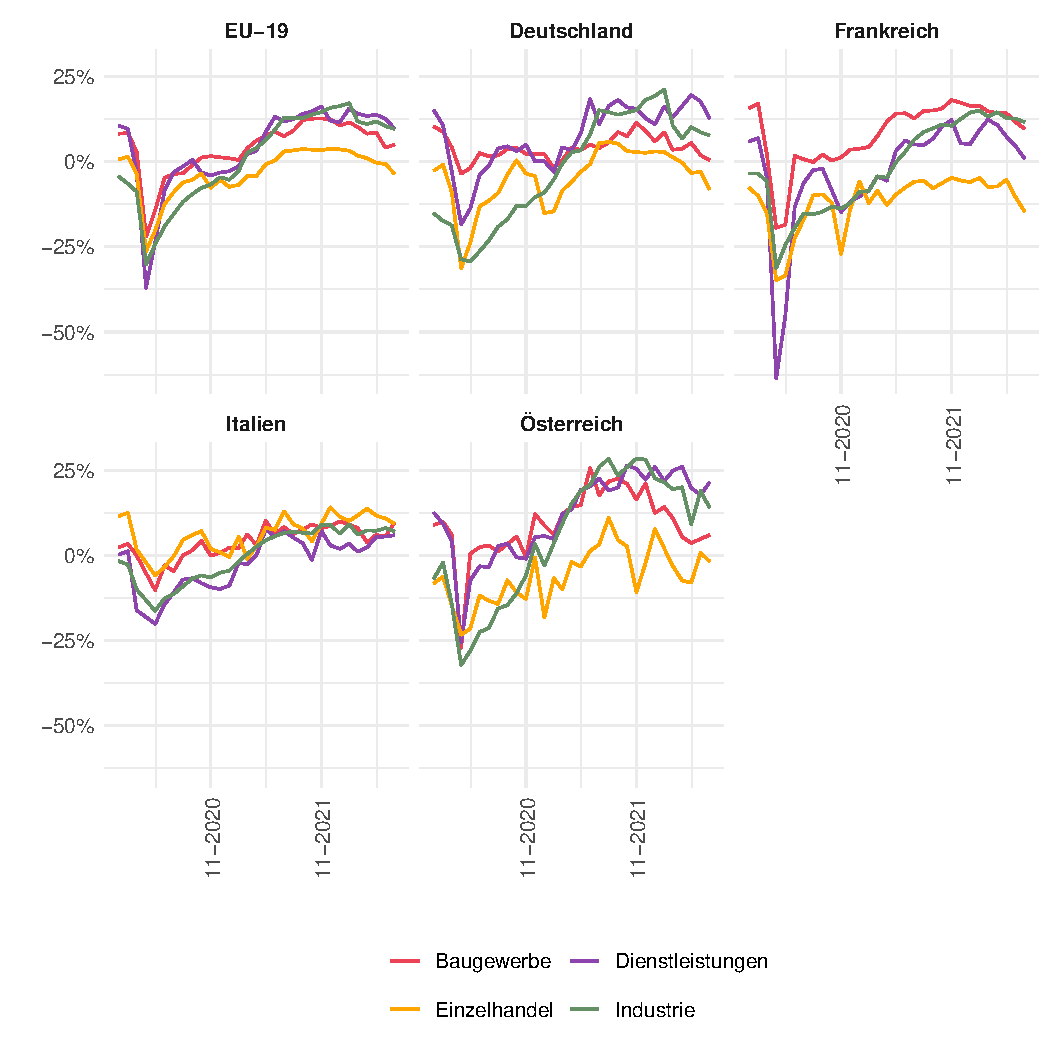
\includegraphics[trim={0 2.5cm 0 0cm },clip,width=\textwidth]
{/Users/simonwey/Repos/Foreign_economics/Graphics/wrap_empl_exp_eco.pdf}
\caption{Sektoren und Branchen: Beschäftigungsaussichten nächste 3 Mt.} 
\label{Inf_M_W}
\end{figure}

\begin{figure}[] \centering
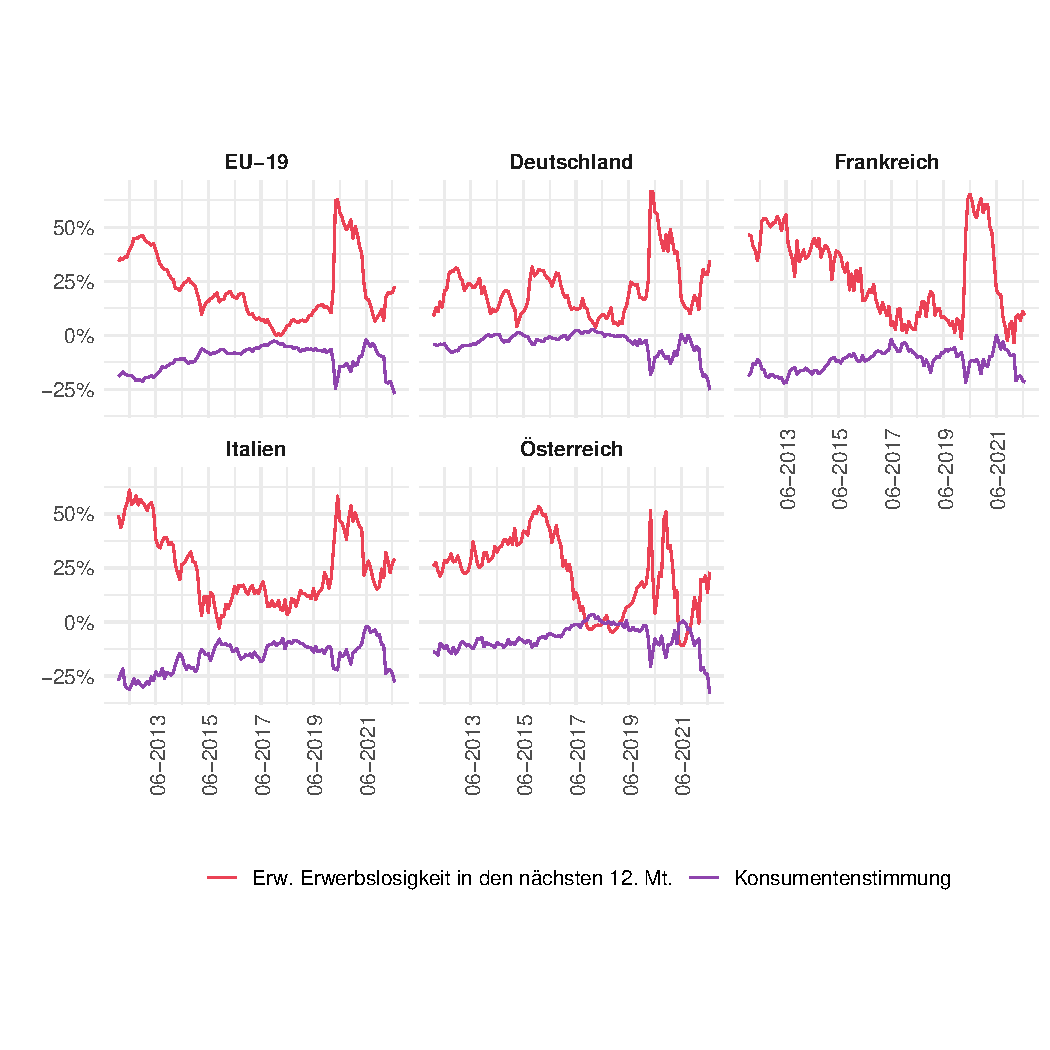
\includegraphics[trim={0 2.5cm 0 0cm },clip,width=\textwidth]
{/Users/simonwey/Repos/Foreign_economics/Graphics/cons_mood.pdf}
\caption{Konsumentenstimmung und Indikator zur Angst, die Stelle in den nächsten 12 Mt. zu verlieren} 
\label{Inf_M_W}
\end{figure}

\begin{figure}[] \centering
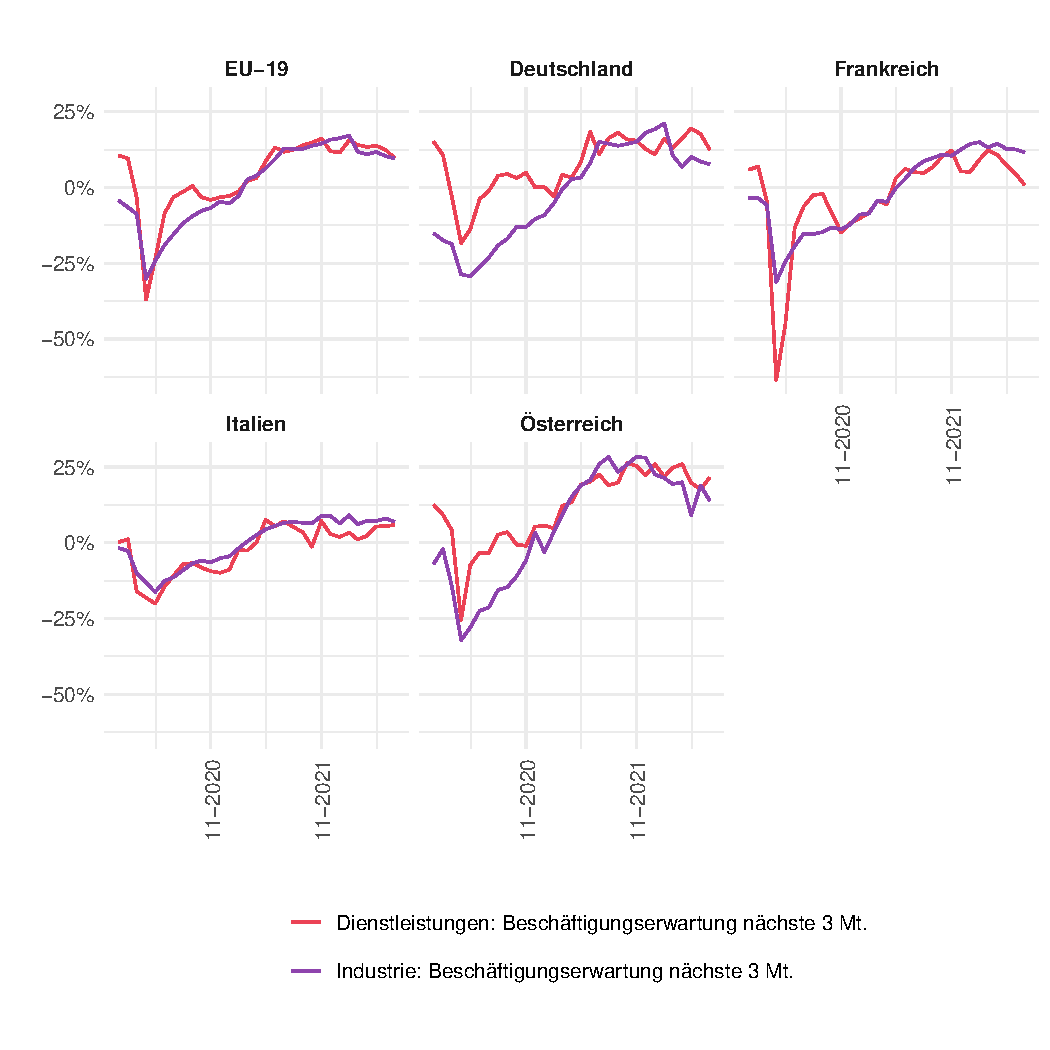
\includegraphics[trim={0 0cm 0 0cm },clip,width=\textwidth]
{/Users/simonwey/Repos/Foreign_economics/Graphics/empl_exp_sector.pdf}
\caption{Beschäftigungserwartungen in der Industrie und dem Dienstleistungssektor} 
\label{Inf_M_W}
\end{figure}

\begin{figure}[] \centering
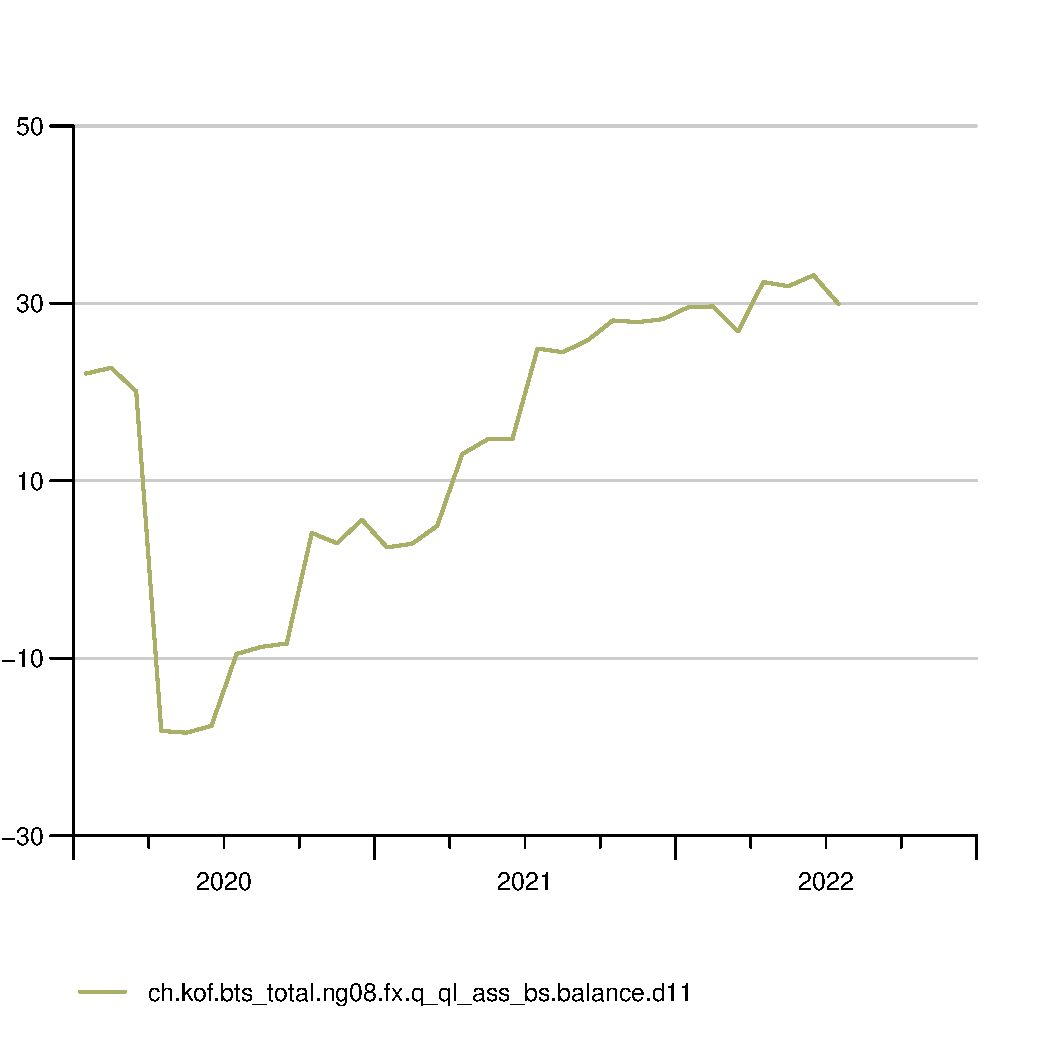
\includegraphics[trim={0 2.5cm 0 0cm },clip,width=.8\textwidth]
{/Users/simonwey/Repos/Foreign_economics/Graphics/GL.pdf}
\caption{Geschäftslagenindikator mit aktuellem Wert 28.4} 
\label{Inf_M_W}
\end{figure}

\begin{longtable}[]{@{}lll@{}}
\caption{Geschäftslageindikator, letzte Werte. Quelle:
KOF}\tabularnewline
\toprule
\textbf{Monat} & \textbf{August} & \textbf{September} \\
\midrule
\endfirsthead
\toprule
\textbf{Monat} & \textbf{August} & \textbf{September} \\
\midrule
\endhead
\textbf{KOF-Geschäftslageindikator} & 28.1 & 28.4 \\
\bottomrule
\end{longtable}

\hypertarget{ausgangslage}{%
\section{Ausgangslage}\label{ausgangslage}}

\begin{figure}[] \centering
\includegraphics[trim={0 0cm 0 0cm },clip,width=\textwidth]
{/Users/simonwey/Repos/Foreign_economics/Graphics/wrap_Hin_both.pdf}
\caption{Hemmnisse Sektoren} 
\label{Inf_M_W}
\end{figure}

\begin{figure}[] \centering
\includegraphics[trim={0 0cm 0 0cm },clip,width=\textwidth]
{/Users/simonwey/Repos/Foreign_economics/Graphics/wrap_Hind_constr.pdf}
\caption{Hemmnisse Bausektor} 
\label{Inf_M_W}
\end{figure}

\end{document}
